\documentclass[12pt, a4paper]{article}
\usepackage{amsmath}
\usepackage{graphicx}
\usepackage{tabularx}
\usepackage{enumerate}
\usepackage{enumitem}
\usepackage[margin=1in]{geometry}
\usepackage[open]{bookmark} %pdf bookmarks
\usepackage{hyperref}
\hypersetup{pdfstartview={XYZ null null 1.00}} % pdf zoom 100%
\usepackage{caption} % these 2 for subfigures
\usepackage{subcaption}
\usepackage{float} % for extra float options such as [H] after \begin{figure}
\linespread{1.3}
\usepackage{titlesec}
\setlength{\parindent}{0pt}
\setlength{\parskip}{1em}
\titlespacing*{\section}{0pt}{0cm}{0cm}
\titlespacing*{\subsection}{0pt}{0cm}{-0.2cm}

\begin{document}
%\title{\vspace{-2.0cm}Cascade Experiment}
%\author{\vspace{-5.0cm}CCN: 5726A}
%\date{\vspace{-2.0cm}26/10/2021}
%\maketitle

\begingroup  
\centering
\LARGE Aviation and the Environment Coursework\\[1em]
\large CCN: 5726A \\
\large 08/12/2021 \\
\endgroup

%\renewcommand{\thesubsection}5{\arabic{subsection}} % Remove section number from subsection numbering
\section{Summary}
Aircraft engines and their cruise operating conditions have been optimised to maximise commercial profits which have led to some focus on fuel efficiency but not on 
their environmental impacts. This coursework asks the question: How could the 
environmental impact be improved by operating aircraft differently? A code is developed to investigate effects of varying cruise altitude and overall pressure ratio (OPR) to help answer this question. Other limits on operating conditions are considered and the need to compromise between cost (fuel burn) and environmental impacts is discussed.

\section{Model}
This coursework was carried out using Python 3.7. The full script can be found in the \hyperref[sec:Appendix]{Appendix}. The atmosphere is modelled with the International Standard Atmosphere (ISA) conditions:
\begin{figure}[H]
	\centering
	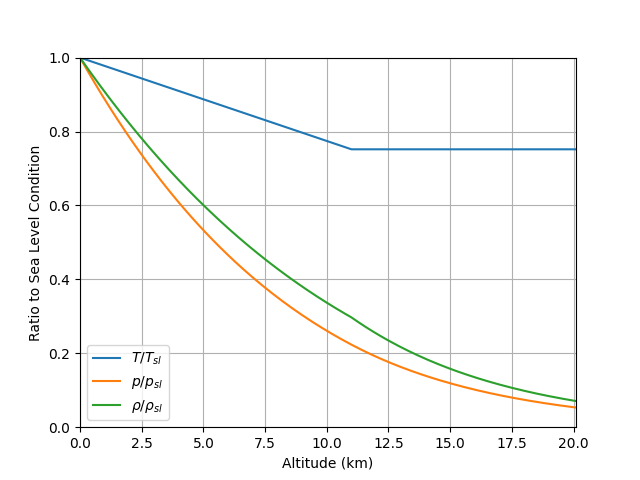
\includegraphics[width=0.65\textwidth]{../Plots/ISA}
	\caption{ISA conditions at different altitudes, plotted with matplotlib}
	\label{fig:isa}
\end{figure} 
A look-up table was created to allow the code to get atmospheric conditions at any altitude. Next, basic reference data of the aircraft and engine were set:
\begin{table}[h]
	\centering
	\caption{Model Reference Data}
	\label{tab:ref}
	\begin{tabular}{|l|c|l|c|}
		\hline
		\multicolumn{2}{|c|}{\textbf{Aircraft}} & \multicolumn{2}{c|}{\textbf{Engine}} \\ \hline
		Number of Passengers: & 240 & Temperature Ratio $\theta$: &  6 \\ \hline
		Range: & 12000 km & Turbine, Compressor Efficiencies $\eta_t,\eta_c$ & 0.9 \\ \hline
		Payload Mass $w_p$: & 40 tonnes & Fan Pressure Ratio \textit{FPR}: & 1.45 \\ \hline
		Empty Mass $w_e$: & 106 tonnes & Fan Efficiency $\eta_f$: & 0.92 \\ \hline
		Initial Fuel Mass $ w_f $: & 74 tonnes & Transfer Efficiency $\eta_{tr}$: & 0.9 \\ \hline
		Take Off Mass $ w_{TO} $: & 220 tonnes & Parabolic drag law constants $ K1 $: & 0.0125\\ \hline
		Wing Area $S$: & 315 $m^2$ &  Parabolic drag law constants $ K2 $: & 0.0446 \\ \hline
	\end{tabular}
\end{table}

\subsection{Multiple Staged Flight}
The flight is split into 10 stages, with all calculated quantities being constant within each stage. Sequence of calculated values are summarised (detailed calculations in \hyperref[sec:Appendix]{Appendix}):

Optimum Equivalent Air Speed (EAS) $\rightarrow$ Actual EAS $\rightarrow$ True Air Speed (TAS) $\rightarrow$ Aircraft Mach $\rightarrow$ Jet Mach $\rightarrow$ Jet Temperature $\rightarrow$ Propulsive Efficiency $\rightarrow$ L/D $\rightarrow$ Range Parameter H $\rightarrow$ New Weight \& Fuel Burnt $\rightarrow$ Emission Indices ($EI_{CO_2}$ \& $EI_{NO_X}$) $\rightarrow$ Total Emissions per stage

After each stage has been iterated, the total fuel burnt and emissions for both Carbon Dioxide ($CO_2$) and Nitrogen Oxides ($NO_X$) are summed up to calculate the overall fuel burnt per passenger-km and emissions per passenger-km. These are the most important quantities that are compared when varying parameters. 

At a flight of $altitude = 9.5km$ and $OPR = 45$, the variation of Mach numbers and emissions during the whole flight can be visualised: 

%\DeclareCaptionSubType*{figure}
\renewcommand{\thesubfigure}{\thefigure\alph{subfigure}}
\renewcommand{\subfigurename}{Figure}
\captionsetup[figure]{belowskip=-1.5cm}
\begin{figure}[H]
	
	\begin{subfigure}[b]{0.5\textwidth}
		\centering
		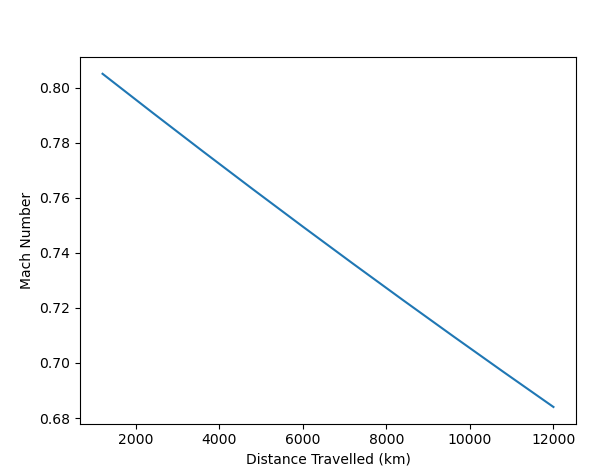
\includegraphics[width=\textwidth]{../Plots/mach 9.5 45}
		\caption{Mach number during flight}
		\label{fig:mach}
	\end{subfigure}
	\hfill
	\begin{subfigure}[b]{0.5\textwidth}
		\centering
		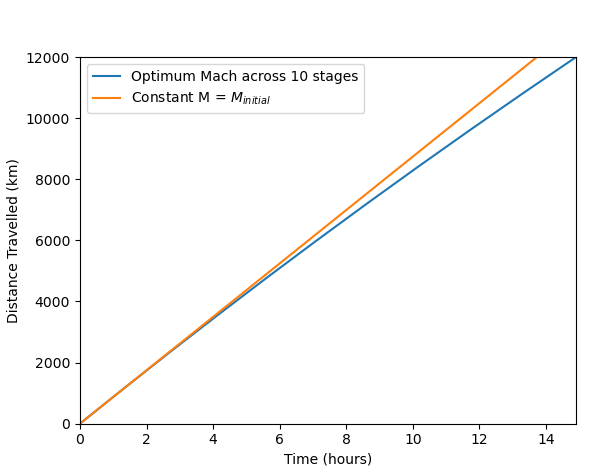
\includegraphics[width=\textwidth]{../Plots/xt diagram 9.5 45}
		\caption{x-t diagram of the whole flight}
		\label{fig:xt}
	\end{subfigure}
	\hfill
\end{figure}


\captionsetup[figure]{aboveskip=-1cm,belowskip=-0.5cm}
\begin{figure}[H]
	\begin{subfigure}[b]{0.5\textwidth}
		\centering
		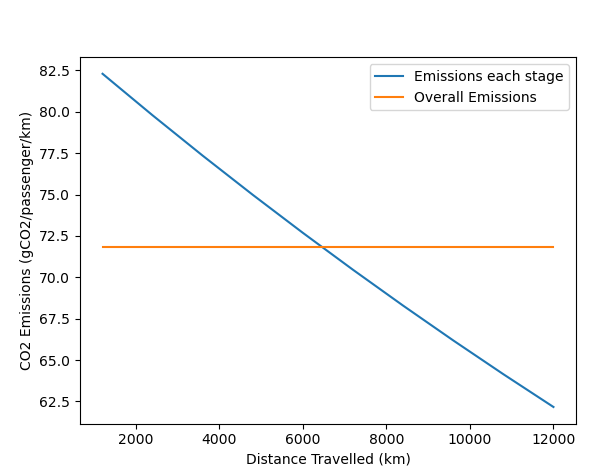
\includegraphics[width=\textwidth]{../Plots/co2 9.5 45}
		\label{fig:co2}
	\end{subfigure}
	\hfill
	\begin{subfigure}[b]{0.5\textwidth}
		\centering
		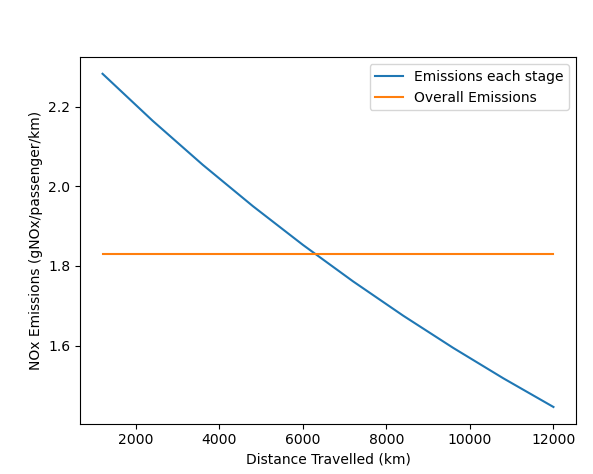
\includegraphics[width=\textwidth]{../Plots/nox 9.5 45}
		\label{fig:nox}
	\end{subfigure}
	\hfill
	\caption{Emissions / pass-km for $CO_2$ and $NO_X$}
	\label{fig:emission}
\end{figure}
\captionsetup[figure]{aboveskip=1pt,belowskip=1pt}
Because the altitude and optimum L/D are fixed, the velocity and Mach number decrease as fuel is burnt. In \hyperref[fig:mach]{Figure 2a}, the Mach number almost decreases linearly. This decrease lengthens the flight duration compared to if the Mach number was kept constant at the initial speed. This can be seen in \hyperref[fig:xt]{Figure 2b}, where the flight duration increases from 13.6 to 14.8 hours.

This optimising of flight speed leads to a decrease in both $CO_2$ and $NO_X$ emissions per passenger-km. In \autoref{fig:emission}, both emissions decrease almost linearly relative to the overall emission per passenger-km. This is evidence for how shorter journeys have a lower emission per passenger-km, because less fuel needs to be carried, leading to lower optimum Mach numbers and hence emissions.

\subsection{Model Limitations}
As weight decreases due to fuel burn, to keep the lift coefficient ($C_L$) constant the velocity or density must decrease. The latter can be done by flying at higher altitudes. In this model, each flight has a fixed cruise altitude and an decreasing flight speed. Whereas in practice flight speed is fixed with an increasing cruise altitude, known as 'cruise climb'. 

Secondly, the calculations for emissions do not take into account 'k' which adjusts the fuel burn equation for the initial take off and climb. However, this is negligible as k is typically 1.5\% for long journeys.

Lastly, this model ignores the effects of transonic drag rise, such as buffeting and shock-induced separations, in the optimum velocity. A check has been implemented to print out a warning if Mach exceeds 0.85, which it can be seen later this occurs for some higher cruise altitudes. This must be considered when analysing the results.

\section{Effects of Cruise Altitude}
Although in the model cruise altitude is fixed for each flight, it can be varied for different flights. Altitudes from 8km to 12.5km are investigated, with OPR fixed at 45.

\subsection{Fuel Burnt} \label{sec:fuel}
\captionsetup[figure]{belowskip=-1.5cm}
\begin{figure}[H]
	\begin{subfigure}[b]{0.5\textwidth}
		\centering
		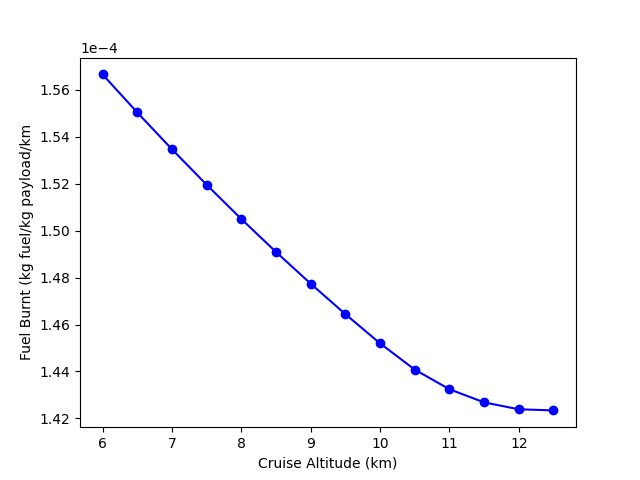
\includegraphics[width=\textwidth]{../Plots/h fuel}
		\caption{Overall fuel burnt}
		\label{fig:hfuel}
	\end{subfigure}
	\hfill
	\begin{subfigure}[b]{0.5\textwidth}
		\centering
		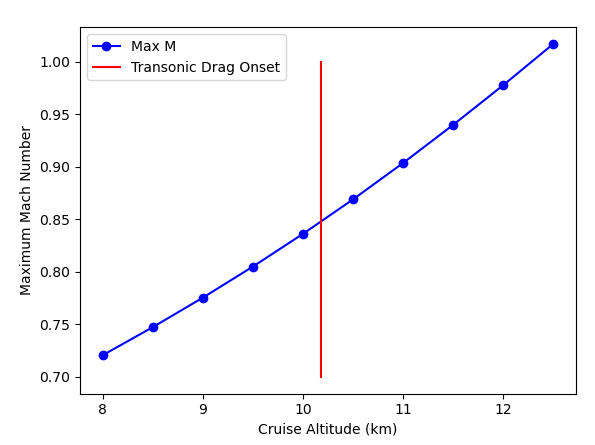
\includegraphics[width=\textwidth]{../Plots/h max m}
		\caption{Maximum Mach number}
		\label{fig:hmach}
	\end{subfigure}
	\label{hfuel}
	\hfill
\end{figure}
\renewcommand{\thesubfigure}{\alph{subfigure}}
\renewcommand{\subfigurename}{}
\captionsetup[figure]{belowskip=-0.5cm}

\hyperref[fig:hfuel]{Figure \thefigure a} suggests that the higher the cruise altitude the better the fuel economy. However, the Mach number also increases due to a lower density and a fixed $C_L$. \hyperref[fig:hfuel]{Figure \thefigure b} shows that the maximum Mach reaches 0.85 at an altitude of 10.2km, where the transonic drag becomes significant. This implies the optimum altitude for fuel economy is just beyond 10.2km, where the drawbacks of transonic drag outweigh the decrease in fuel burnt. This agrees with practice, which places this optimum height at 35000ft, or 10.8km. 

One might make the assumption that lower fuel burnt means lower $CO_2$ and $NO_X$ emissions. However, not only does altitude affect the atmospheric temperature, hence $T_{03}$ and the $NO_X$ emission index ($EI_{NO_X}$), but more significantly the Global Warming Potential (GWP) also scales with height.

\subsection{Global Warming Potential}
GWP describes the relative global warming impacts of 1 tonne of a greenhouse gas relative to 1 tonne of $CO_2$. Svennson et al. (2004) quantified the GWP of $NO_X$ for varying altitudes. \autoref{fig:gwp} shows that the impacts of $NO_X$ are significant around $h=8km$ to $12km$, 50-60 times larger than $CO_2$. However, this is the impacts of the same mass of gas, in our analysis it can be seen that the amount of $NO_X$ produced is also a magnitude smaller than $CO_2$.
\begin{figure}
	\centering
	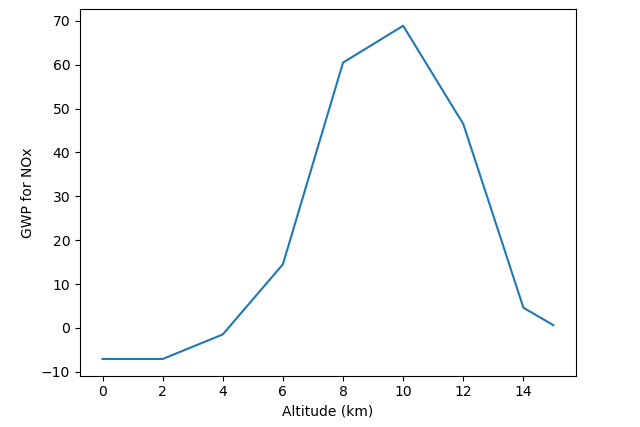
\includegraphics[width=0.5\textwidth]{../Plots/GWP svensonn}
	\caption{Svennson et al.'s GWP of $NO_X$ relative to $CO_2$}
	\label{fig:gwp}
\end{figure} 
\subsection{Emissions and GWP}
\begin{figure}[H]
	\centering
	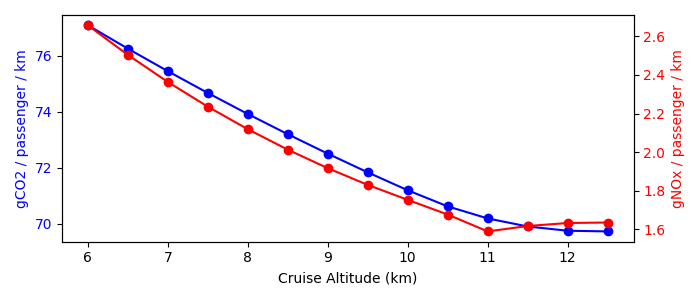
\includegraphics[width=0.9\textwidth]{../Plots/h1}
	\caption{Emissions per passenger-km against altitude}
	\label{fig:h1}
\end{figure}
\autoref{fig:h1} shows that increasing altitudes decreases both gases' emissions but up to $11km$ for $NO_X$. $CO_2$ follows the same trend as fuel burnt because $EI_{CO_2}$ is constant at $3088gCO_2/kg fuel$. Above $11km$ the atmospheric temperature is constant, which with an increasing velocity means $T_{02}$, $T_{03}$ and $EI_{NO_X}$ all increase. Below 11km the lower temperature outweighs the higher velocity, leading to an overall lower emission. This explains the discontinuity at $11km$. To understand the full impact of these emissions, the GWP from \autoref{fig:gwp} is multiplied to the $NO_X$ emissions:
\begin{figure}[H]
	\centering
	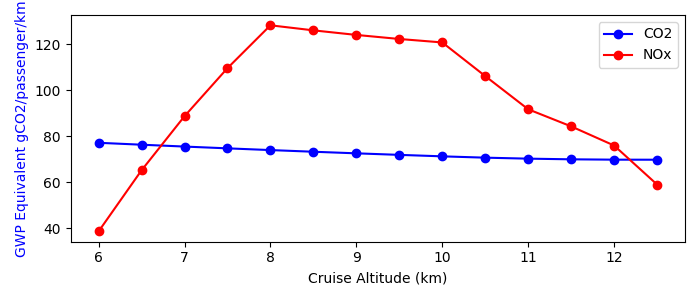
\includegraphics[width=0.85\textwidth]{../Plots/h2}
	\caption{GWP Equivalent $gCO_2/passenger-km$}
	\label{fig:h2}
\end{figure}
\begin{figure}[H]
	\centering
	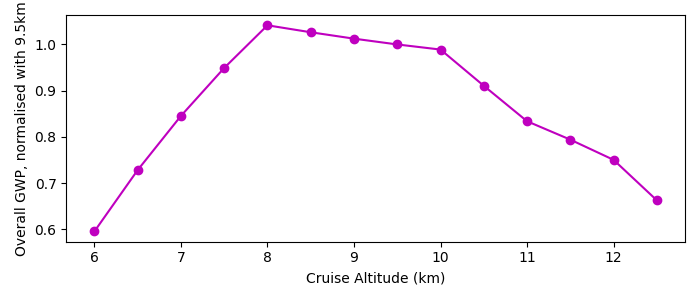
\includegraphics[width=0.85\textwidth]{../Plots/h3}
	\caption{Overall GWP normalised with $h=9.5km$}
	\label{fig:h3}
\end{figure}
The GWP of both emissions are summed up in \autoref{fig:h3}, where it is normalised with the value at $9.5km$. It can be seen that the global warming effects are the  highest around $8-10km$, dropping rapidly on either side. This is due to the GWP of $NO_X$ (\autoref{fig:gwp}) being the more dominating factor. The high levels of emissions at low altitude (and later increasing $NO_X$ past 11km) are outweighed by the negligible relative global warming effects at these altitudes. Ideally the cruise altitude should be very low or very high, but limitations of transonic drag and minimum altitude apply, which will be discussed in \ref{sec:c1}.

\section{Effects of Engine Overall Pressure Ratio}
OPR from 20 to 55 are investigated, with cruise altitude fixed at 9.5km.
\subsection{Fuel Burnt}
\begin{figure}
	\centering
	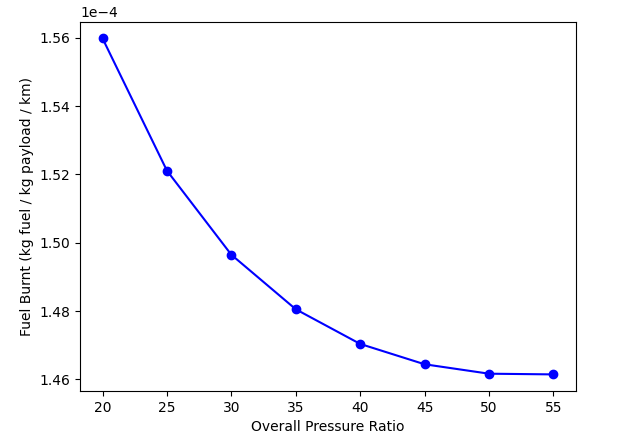
\includegraphics[width=0.55\textwidth]{../Plots/opr fuel}
	\caption{Overall fuel burnt}
	\label{fig:ofuel}
\end{figure}

The cycle efficiency increases as OPR increases, leading to a  decreasing overall fuel burnt. This decrease levels off at $OPR=55$ as seen in \autoref{fig:o1}. The optimum OPR for fuel economy is at the highest OPR possible, limited by current technology (discussed later).

\subsection{Emissions and GWP}
\begin{figure}[H]
	\centering
	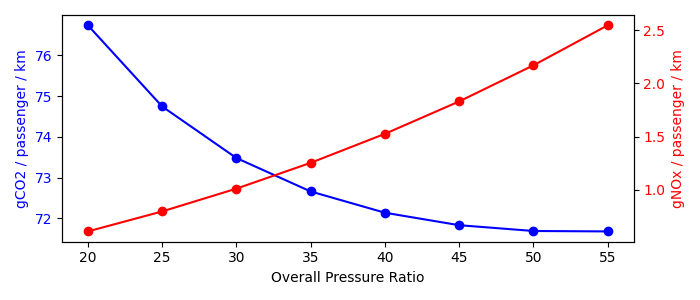
\includegraphics[width=0.9\textwidth]{../Plots/opr1}
	\caption{Emissions per passenger-km against OPR}
	\label{fig:o1}
\end{figure}
The $CO_2$ emissions follow the same trend as fuel burnt because $EI_{CO_2}$ is constant at $3088gCO_2/kg fuel$. The $NO_X$ emissions have an opposite trend which increases as OPR increases. This is a result of a higher compressor exit temperature, hence $T_{03}$ and $EI_{NO_X}$. The higher $EI_{NO_X}$ exceeds the lower fuel burnt. To understand the full impact of these emissions, a $GWP=66.8$ at $9.5km$ from \autoref{fig:gwp} is multiplied to $NO_X$ emissions:

\begin{figure}[H]
	\centering
	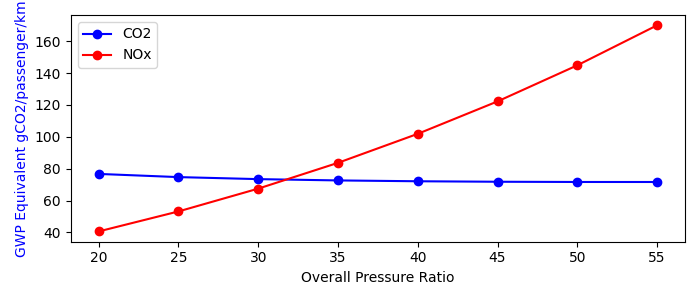
\includegraphics[width=0.8\textwidth]{../Plots/opr2}
	\caption{GWP equivalent g$CO_2$/passenger-km}
	\label{fig:o2}
\end{figure}
\begin{figure}[H]
	\centering
	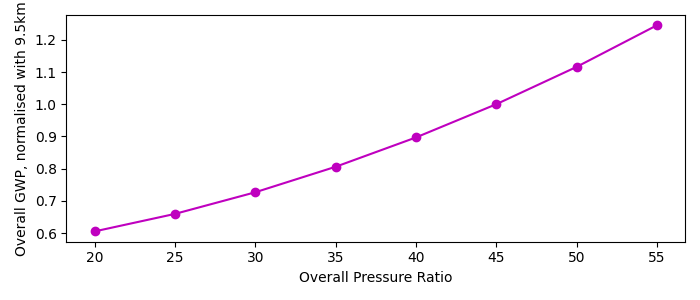
\includegraphics[width=0.8\textwidth]{../Plots/opr3}
	\caption{Overall GWP normalised with OPR=45}
	\label{fig:o3}
\end{figure}

Combining the global warming effects of both gases shows that the overall effects are dominated by the $NO_X$ at high OPR. In \autoref{fig:o3} the lower the OPR, the lower the overall global warming impacts the emissions have. This concludes that the optimum OPR for the environment is at the lowest OPR possible. However, this contradicts the optimum OPR for fuel economy, and this will be discussed in the next section. Moreover, the altitude was set at 9.5km, where the GWP of $NO_X$ is significant. Therefore, it is worthwhile to run the same model for all altitudes and OPR.

\section{Optimum Operating Points}
By running the program for altitudes from $6-13.5km$ and OPR from $10-55$, contours for the overall global warming potential and fuel burnt are visualised. This allows the best operating points to be identified. This will show what is best for the environment versus what is best in terms fuel burnt and hence cost.

\subsection{The Environment} \label{sec:c1}
\begin{figure}
	\centering
	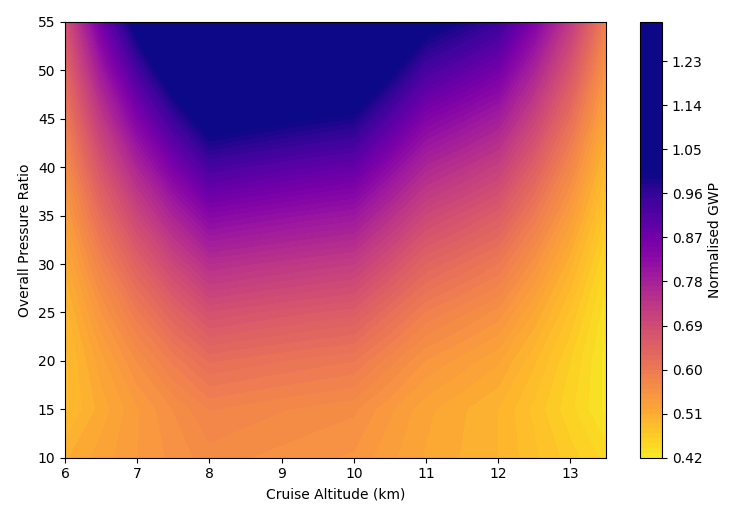
\includegraphics[width=\textwidth]{../Plots/contour ovr}
	\caption{Contour of overall GWP, normalised with $h=9.5km$, $OPR=45$}
	\label{fig:c1}
\end{figure}
\autoref{fig:c1} shows that the best operational points for the environment lie in regions of low OPR, at very high or very low altitudes. However, the maximum altitude is limited by the onset of transonic wave drag, which occurs at around $10.8km$ as discussed in section \ref{sec:fuel}. Above this altitude the extra emissions due to transonic drag starts to dominate the lower GWP due to altitude. Secondly, the minimum altitude is limited by mountain ranges, for example the Himalayan mountain ranges can reach up to 9km. This lower limit means the GWP at $9km$ is greater than the GWP at the upper limit of $10.8km$. The minimum OPR is limited by the net work output, or thrust, the engine produces. For temperature ratio of $\theta=6$, the non-dimensionalised specific power drops abruptly below $OPR=15$. To conclude, the optimum operating condition to minimise overall global warming effects: \underline{\text{\boldmath$OPR = 15$} \textbf{and}  \text{\boldmath$altitude=11km$}}. 

However, for flight paths that do not cross high mountain ranges, it is also worth operating at low altitudes for a similar reduced GWP. This is especially applicable to short flights where the relative fuel burn due to climbing to high altitudes becomes significant.

\subsection{The Costs}
The operating condition found in the previous section assumes airliners have the environment's best interests in mind. However, fuel burnt is directly related to operating costs. 
\begin{figure}
	\centering
	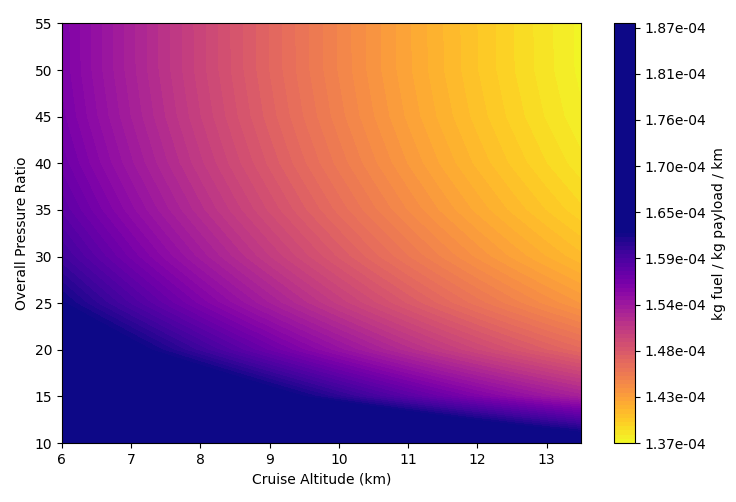
\includegraphics[width=0.8\textwidth]{../Plots/contour fuel}
	\caption{Contour of overall fuel burnt, normalised with h=9.5km, OPR=45}
	\label{fig:c2}
\end{figure}
A contour is plotted for the overall fuel burnt in \autoref{fig:c2}. This shows the optimum operating condition for fuel economy is at the highest altitude and OPR possible. The maximum altitude is once again limited by transonic drag, but now the maximum OPR is limited by the material's thermal properties and number of compressor stages required. This places the limit at 55-60. 

With this in mind, airliners must compromise between mitigating environmental impacts by flying at low OPR, and minimising costs by flying at high OPR. At the moment the focus is on the latter, hence the development of high OPR engines, but with the right governmental and societal shift airliners could easily fly at lower OPR in favour of the environment. The optimum altitude for  environmental and costs is both at the highest altitude allowed by the onset of transonic wave drag. 

\subsection{Other Operating Conditions and Technology}
Other conditions such as temperature ratio $\theta$ and using 'short hops' for long flights could also be utilised to mitigate global warming effects. The latter was seen briefly in \hyperref[fig:mach]{Figure 2a} and \autoref{fig:emission}, where shorter journeys reduce fuel burnt and emissions significantly. Technological advancements to improve various efficiencies in the engine and propeller, as well as aerodynamic designs to increase L/D, could also contribute to reducing emissions. Lastly, alternative fuels such as hydrogen and electricity are also means to reduce GWP.

\section{Conclusion}
A code was developed in Python to analyse the $CO_2$ and $NO_X$ emissions as well as their relative global warming impacts for various cruise altitudes and OPR. Each flight had a fixed altitude, leading to an increasing Mach and decreasing emissions throughout the flight. Flying at higher altitudes decreased the amount of fuel burnt and emissions. Due to significant GWP of $NO_X$ at mid-range cruise altitudes, the overall GWP for $CO_2$ and $NO_X$ were lowest outside 8-10km. Flying at higher OPR decreased the amount of fuel burnt but levelled off at 50. $CO_2$ and $NO_X$ had opposite emission trends with OPR, but $NO_X$ dominated in terms of overall GWP. A contour of overall GWP was plotted for all altitudes and OPR, the optimum operating condition was at $OPR=15$ and $altitude=11km$. Maximum  and minimum altitudes are limited by transonic wave drag and mountain ranges respectively, and minimum OPR limited by thrust required. A compromise between the environment (low OPR) and cost (high OPR) must be made.

\newpage
\section{Appendix}\label{sec:Appendix}
\subsection{Detailed Calculations in Python Iteration}
\begin{enumerate}[label=\roman*.]
	\item Optimum Equivalent Air Speed (EAS) = $ V^*_e=\left[ \dfrac{mg}{0.5\rho_0S}\right]^{0.5}\left[\dfrac{K_2}{K_1}\right]^{0.25} $
	\item Actual EAS = $ V_e=V^*_e \times \nu $ , where $\nu=1$ is the selected speed ratio  
	\item True Air Speed (TAS) = $ V=V_e\,\sqrt{\rho_0/\rho_a} $
	\item Mach Number $M=V/a$, where $a$ is the local speed of sound
	\item Jet Mach $M_j^2=\dfrac{2}{\gamma-1}\left[(FPR\times p_{02}/p_a)^{(\gamma-1)/\gamma}-1\right]$
	\item Jet Temperature $ \dfrac{T_j}{T_a}=\dfrac{1+0.5(\gamma-1)M^2}{1+0.5(\gamma-1)M_j^2}FPR^{(\gamma-1)/(\gamma\,\eta_f)} $
	\item Propulsive Efficiency $ \eta_{prop}=2\,\left(1+M_j/M \;\sqrt{T_j/T_a}\right)^{-1} $
	\item $ L/D=\left(\sqrt{K_1\,K_2}\,(\nu^2+1/\nu^2)\right)^{-1} $
	\item Range Parameter $ H=\eta_{prop}\,\eta_{cycle}\,\eta_{tr}\,L/D\times LCV/g $
	\item New Weight $ w_{end} = w_{start} \, e^{s_{stage}/H} $
	\item $EI_{CO_2}=3088$, $ EI_{NO_X}=0.011445\,e^{0.006766\times T_{03}} $, where $T_{03}=T_{02}\times \left(1+(OPR^{(\gamma-1)/\gamma}/\eta_c)\right)$
	\item Total Emissions for this stage $ = EI\,\times \, Fuel\;Burnt$
\end{enumerate}
\subsection{Full Python Script}
\textbf{NOTE: Change h and OPR in lines 82-85, then comment/uncomment corresponding plots starting at lines 192 (vary h) 264 (vary OPR) 296 (contour)}

\end{document}
